\documentclass[12pt,a4paper]{article}
\raggedbottom

\usepackage{ugmath}
\usepackage{float}
\usepackage{placeins}
\usepackage[labelfont=bf,labelsep=space]{caption}
\usepackage{pdfpages}
\usepackage{tikz-cd}
\usepackage{amsthm}
\renewcommand{\Tr}{\operatorname{Tr}}
\newcommand{\llaves}[1]{\{#1\}}
\newcommand{\parentesis}[1]{\left(#1\right)}
\newcommand{\corchetes}[1]{\left[#1\right]}
\newcommand{\llavesgrande}[1]{\big\{#1\big\}}
\newcommand{\llavesgrandes}[1]{\left\{#1\right\}}


\begin{document}
        
    
    \thispagestyle{empty}
    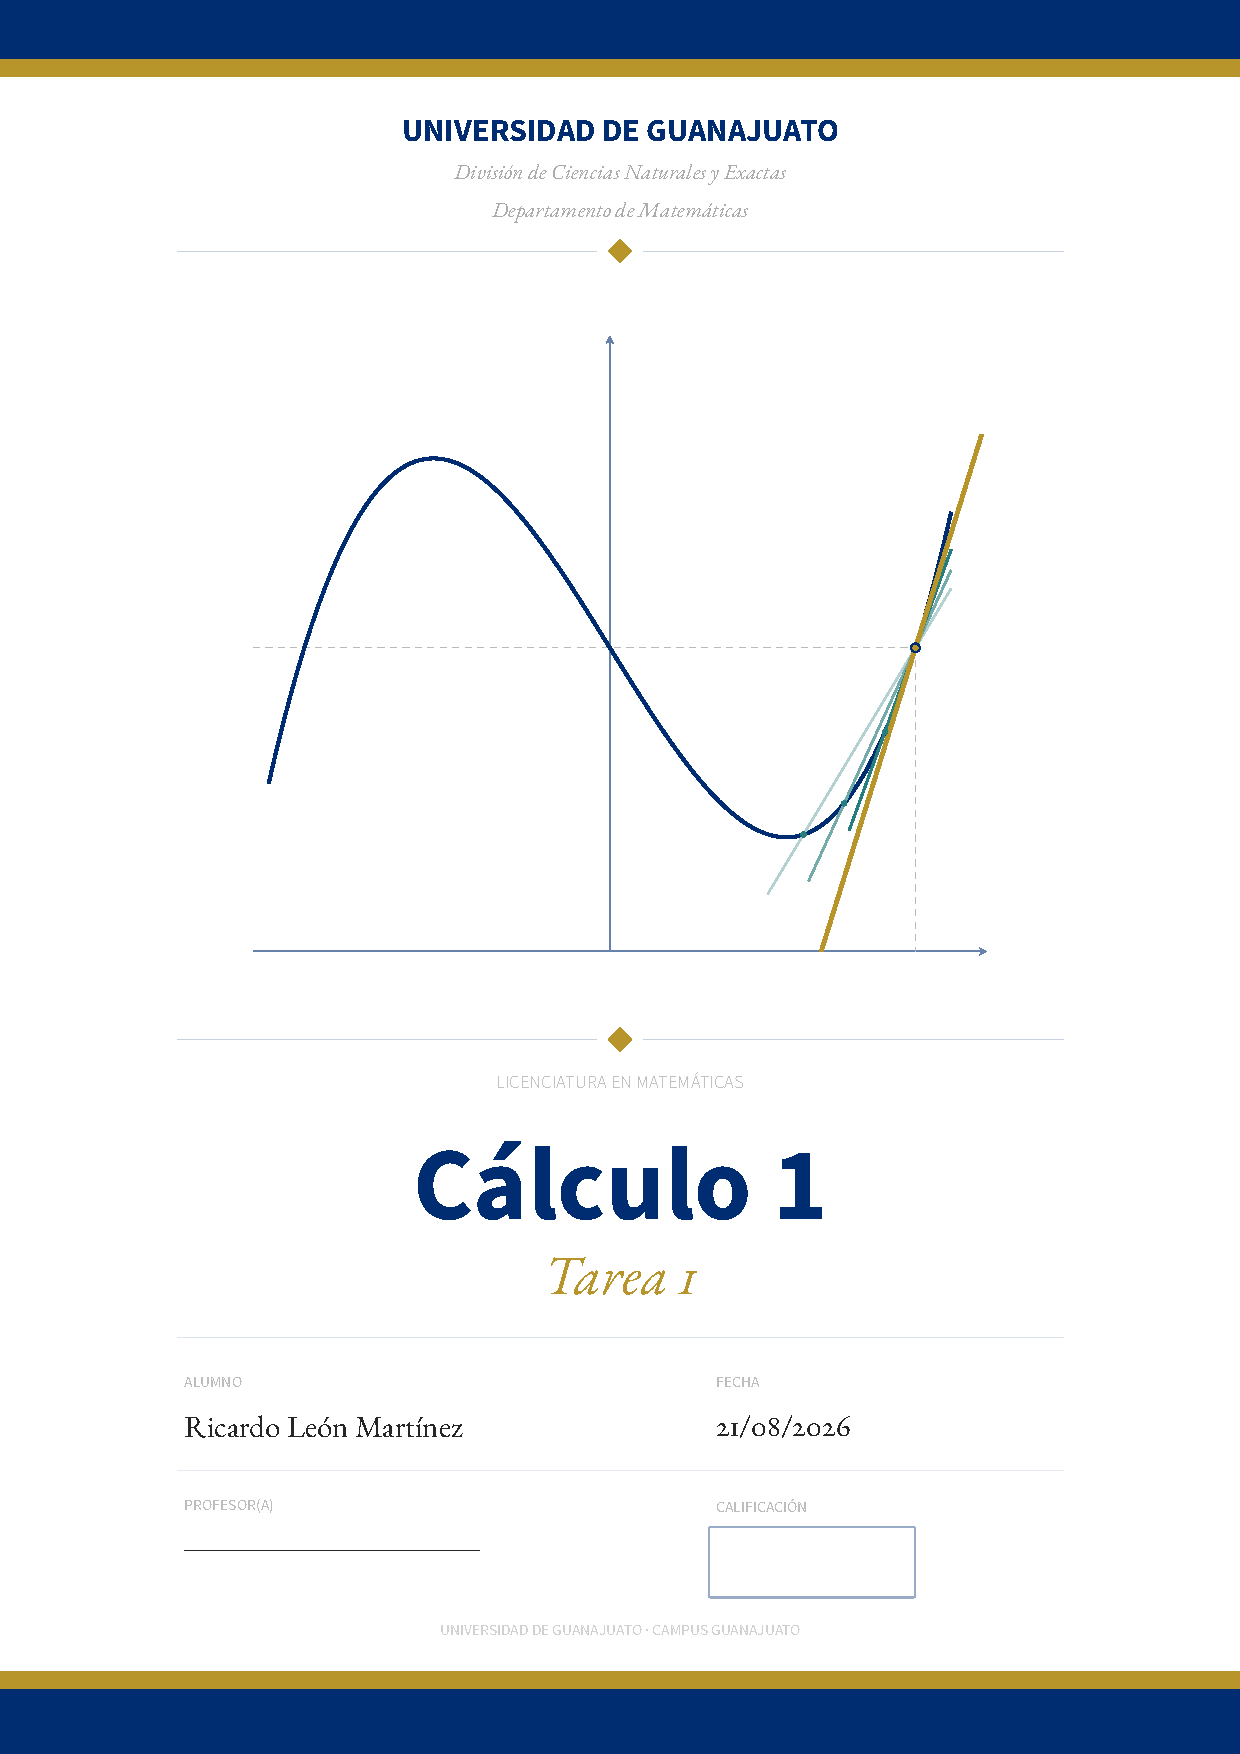
\includepdf[pages=1]{main.pdf}

    \begin{problema}
        Expresa los conjuntos siguientes mediante alguna condición.
        \begin{multicols}{2}
            \begin{enumerate}
                \item[(a)] $\{1,3,5,7,\dots\}$.
                \item[(b)] $\{2,4,6,8,\dots\}$.
                \item[(c)] $\{9,10,11,12,\dots\}$.
                \item[(d)] $\{7,8,\dots,93,94\}$.
                \item[(e)] $\{1,2,4,8,16,\dots\}$.
                \item[(f)] $\{1,1/2,1/3,1/4,\dots\}$.   
            \end{enumerate}
        \end{multicols}
    \end{problema}

    \begin{solucion}
        \begin{multicols}{2}
            \begin{enumerate}
            \item[(a)] $\{1,3,5,7,\dots\}=\{2n-1:n\in\N\}$.
            \item[(b)] $\{2,4,6,8,\dots\}=\{2n:n\in\N\}$.
            \item[(c)] $\{9,10,11,12,\dots\}=\{n\in\N: n\geq9\}$.
            \item[(d)] $\{7,8,\dots,93,94\}=\{n\in\N:7\leq n\leq94\}$.
            \item[(e)] $\{1,2,4,8,16,\dots\}=\{2^{n}:n\in\N\cup\{0\}\}$.
            \item[(f)] $\{1,1/2,1/3,1/4,\dots\}=\left\{\frac{1}{n}:n\in\N\right\}$.  
            \end{enumerate}            
        \end{multicols}
    \end{solucion}

    \begin{problema}
        Sean $A=\{0,1,2,3,4,5,6,7,8,9\}$, $B=\{5,6,7,8,9\}$, $C=\{0,1,2,3,4\}$, $D=\{3,4,5\}$ y
        $E=\{a,e,i,o,u\}$ y $F=\{a,e,o\}$. Calcula lo siguiente:
        \begin{multicols}{2}
            \begin{enumerate}
                \item[(a)] $A\cup B$, $B\cup C$ y $D\cup F$.
                \item[(b)] $A\cap B$, $B\cap C$ y $D\cap F$. 
                \item[(c)] $B\cup C\cup D$ y $B\cap C\cap D$.
                \item[(d)] $B\cup D\cup E$ y $B\cap D\cap E$.
                \item[(e)] $A\setminus B$, $B\setminus A$, $B\setminus C$ y $A\setminus D$.  
                \item[(f)] $A\setminus E$, $E\setminus A$, $E\setminus F$ y $F\setminus E$. 
            \end{enumerate}
        \end{multicols}
    \end{problema}

    \begin{solucion}
        \begin{enumerate}
            \item[(a)] $A\cup B$, $B\cup C$ y $D\cup F$.
            \begin{equation*}
                A\cup B=\{0,1,2,3,4,5,6,7,8,9\},\quad B\cup C=\{0,1,2,3,4,5,6,7,8,9\},\quad D\cup F=\{3,4,5,a,e,o\}.
            \end{equation*}
            \item[(b)] $A\cap B$, $B\cap C$ y $D\cap F$.
            \begin{equation*}
                A\cap B=\{5,6,7,8,9\},\quad B\cap C=\varnothing,\quad D\cap F=\varnothing.
            \end{equation*}
            \item[(c)] $B\cup C\cup D$ y $B\cap C\cap D$.
            \begin{equation*}
                B\cup C\cup D=\{0,1,2,3,4,5,6,7,8,9\},\quad B\cap C\cap D=\varnothing.
            \end{equation*}
            \item[(d)] $B\cup D\cup E$ y $B\cap D\cap E$.
            \begin{equation*}
                B\cup D\cup E=\{3,4,5,6,7,8,9,a,e,i,o,u\},\quad B\cap D\cap E=\varnothing
            \end{equation*}
            \item[(e)] $A\setminus B$, $B\setminus A$, $B\setminus C$ y $A\setminus D$.
            \begin{equation*}
                A\setminus B=\{0,1,2,3,4\},\quad B\setminus A=\varnothing,\quad B\setminus C=\{5,6,7,8,9\},\quad A\setminus D=\{0,1,2,6,7,8,9\}
            \end{equation*}
            \item[(f)] $A\setminus E$, $E\setminus A$, $E\setminus F$ y $F\setminus E$.
            \begin{equation*}
                A\setminus E=\{0,1,2,3,4,5,6,7,8,9\},\quad E\setminus A=\{a,e,i,o,u\},\quad E\setminus F=\{i,u\},\quad F\setminus E=\varnothing
            \end{equation*}
        \end{enumerate}
    \end{solucion}

    \begin{problema}
        Encuentra $\bigcup_{n=1}^{\infty}A_{n}$ y $\bigcap_{n=1}^{\infty}A_{n}$ si $A_{n}=\{1,2,\dots,n\}$
        para cada $n\in\N$.
    \end{problema}

    \begin{proof}
        Sea $x\in\bigcup_{n=1}^{\infty}A_{n}$. Por definición de la unión, existe $n\in\N$ tal que $x\in A_{n}$.
        Como
        \begin{equation*}
            A_{n}=\{1,2,\dots,n\},
        \end{equation*}
        se sigue que $x$ es uno de los números $1,2,\dots,n$. En particular, $x\in\N$. Por lo tanto
        \begin{equation*}
            \bigcup_{n=1}^{\infty}A_{n}\subseteq\N.
        \end{equation*}
        Sea $x\in\N$. Tomemos $n=x$. Entonces
        \begin{equation*}
            A_{x}=\{1,2,\dots,x\}.
        \end{equation*}
        Claramente $x\in A_{x}$. Por definición de unión,
        \begin{equation*}
            x\in\bigcup_{n=1}^{\infty}A_{n}.
        \end{equation*}
        Por consiguiente,
        \begin{equation*}
            \N\subseteq\bigcup_{n=1}^{\infty}A_{n}.
        \end{equation*}
        Concluimos que
        \begin{equation*}
            \bigcup_{n=1}^{\infty}A_{n}=\N.
        \end{equation*}
        Sea
        \begin{equation*}
            x\in\bigcap_{n=1}^{\infty}A_{n}.
        \end{equation*}
        Por definición de intersección, $x\in A_{n}$ para todo $n\in\N$. En particular, tomando $n=1$,
        \begin{equation*}
            x\in A_{1}=\{1\}.
        \end{equation*}
        Luego $x=1$. Por tanto,
        \begin{equation*}
            \bigcap_{n=1}^{\infty}A_{n}\subseteq\{1\}.
        \end{equation*}
        Sea $x=1$. Para todo $n\in\N$,
        \begin{equation*}
            1\in A_{n}=\{1,2,\dots\}.
        \end{equation*}
        Por definición de intersección,
        \begin{equation*}
            1\in\bigcap_{n=1}^{\infty}A_{n}.
        \end{equation*}
        Así,
        \begin{equation*}
            \{1\}\in\bigcap_{n=1}^{\infty}A_{n}.
        \end{equation*}
        Concluimos que
        \begin{equation*}
            \bigcap_{n=1}^{\infty}A_{n}=\{1\}.
        \end{equation*}
    \end{proof}

    \begin{problema}
        \textbf{(El producto cruz de dos conjuntos no es conmutativo)}\\
        Muestra un par de conjuntos $A$ y $B$ tales que $A\times B\neq B\times A$.
    \end{problema}

    \begin{solucion}
        Sea $A=\{1,2\}$ y $B=\{3\}$. Entonces,
        \begin{equation*}
            A\times B=\{(1,3),(2,3)\},\qquad B\times A=\{(3,1),(3,2)\}.
        \end{equation*}
        Así,
        \begin{equation*}
            A\times B\neq B\times A.
        \end{equation*}
    \end{solucion}

    \begin{problema}
        \textbf{(Unicidad del conjunto vacío)}
        Prueba que el conjunto vacío es el único conjunto sin elementos. \textbf{Sugerencia:} Procede por contradicción.
    \end{problema}

    \begin{proof}
        Supongamos que $A$ es un conjunto sin elementos. Entonces para toda $x$, $x\notin A$.
        Para probar que $A\subseteq\varnothing$, sea $x\in A$. Esto es imposible, pues $A$ no tiene
        elementos. Luego la implicación
        \begin{equation*}
            x\in A\implies x\in\varnothing
        \end{equation*}
        es verdadera para todo $x$, y por lo tanto $A\subseteq\varnothing$. Por la proposición 1,
        $\varnothing\subseteq A$. En consecuencia, por el criterio de la igualadad de conjuntos $A=\varnothing$.
        Por lo tanto, el conjunto vacío es único.
    \end{proof}

    \begin{problema}
        Prueba los incisos (b) de la proposición 2.
    \end{problema}

    \begin{proof}
        \begin{enumerate}
            \item[(b)] De la serie de implicaciones
            \begin{align*}
                x\in A\cup(B\cup C)&\implies x\in A\lor(x\in B\lor x\in C)\\
                &\implies (x\in A\lor x\in B)\lor x\in C\\
                &\implies x\in(A\cup B)\cup C
            \end{align*}
            obtenemos que $A\cup(B\cup C)\subseteq (A\cup B)\cup C$. Es fácil ver que las implicaciones
            que aparecen también se cumplen en el sentido contrario, de lo cual obtenemos que $(A\cup B)\cup C\subseteq A\cup(B\cup C)$
            y, en consecuencia, que $A\cup(B\cup C)=(A\cup B)\cup C$. La prueba de que $A\cap(B\cap C)=(A\cap B)\cap C$
            es similar.
        \end{enumerate}
    \end{proof}

    \begin{problema}
        Prueba el inciso (a) la proposición 3
    \end{problema}

    \begin{proof}
        \begin{enumerate}
            \item[(a)] De la serie de implicaciones
            \begin{align*}
                x\in A\cup\varnothing&\implies x\in A\lor x\in\varnothing\\
                &\implies x\in A
            \end{align*}
            obtenemos que $A\cup\varnothing\subseteq A$. Si $x\in A$ por definción es claro que $x\in A\cup\varnothing$.
            En consecuencia $A\subseteq A\cup\varnothing$ y, por lo tanto,
            \begin{equation*}
                A\cup\varnothing=A.
            \end{equation*}
            Sea ahora $x\in A\cap\varnothing$.
            Entonces, por definición de intersección, $x\in A$ y $x\in\varnothing$. Pero $x\in\varnothing$ es imposible,
            ya que el conjunto vacío no tiene elementos. Por lo tanto, no existe ningún $x$ tal que $x\in A\cap\varnothing$.
            En consecuencia, $A\cap\varnothing$ no tiene elementos, es decir,
            \begin{equation*}
                A\cap\varnothing=\varnothing.
            \end{equation*}
            De la serie de implicaciones,
            \begin{align*}
                x\in A\setminus\varnothing&\implies x\in A\wedge x\notin\varnothing\\
                &\implies x\in A
            \end{align*}
            obtenemos que $A\setminus\varnothing\subseteq A$. Si $x\in A$ por definición es claro que
            $x\in A\setminus\varnothing$ y, en consecuencia, $A\subseteq A\setminus\varnothing$. Por lo
            tanto
            \begin{equation*}
                A\setminus\varnothing=A.
            \end{equation*}
            Sea $x\in \varnothing\setminus A$. Entonces por definición de diferencia de conjuntos, $x\in\varnothing\wedge x\notin A$.
            Pero $x\in\varnothing$ es imposible, ya que el conjunto vacío no tiene elementos. Por lo tanto,
            no existe ningún $x$ tal que $x\in \varnothing\setminus A$. En consecuencia, $\varnothing\setminus A$
            no tiene elementos, es decir,
            \begin{equation*}
                \varnothing\setminus A=\varnothing.
            \end{equation*}
        \end{enumerate}
    \end{proof}

\end{document}